\documentclass[11pt]{article}
\usepackage[utf8]{inputenc}
\usepackage[english]{babel}
\usepackage{amsmath}
\usepackage{graphicx}
\usepackage{float}
\usepackage{lipsum}
\usepackage{multicol}
\usepackage{tabularx}
\usepackage{booktabs}
\usepackage{hyperref}
\usepackage{float}
\usepackage{stfloats}
\usepackage{placeins}
\usepackage{wrapfig}
\usepackage{caption}
\usepackage[absolute,overlay]{textpos}
\usepackage[table,xcdraw]{xcolor}
\setlength{\TPHorizModule}{1cm} % Horizontal unit (adjust as needed)
\setlength{\TPVertModule}{1cm}  % Vertical unit (adjust as needed)
\newcolumntype{Y}{>{\centering\arraybackslash}X}
\usepackage[left=2.00cm, right=2.00cm, top=2.00cm, bottom=2.00cm]{geometry}
\title{AN2DL Second Homework Report}

\begin{document}
    
    \begin{figure}[H]
        \raggedright
        
\includegraphics[scale=0.4]{polimi.png} \hfill 
\includegraphics[scale=0.3]{airlab.jpeg}
    \end{figure}
    
    \vspace{5mm}
    
    \begin{center}
        % Select between First and Second
        {\Large \textbf{AN2DL - Second Homework Report}}\\
        \vspace{2mm}
        % Change with your Team Name
        {\Large \textbf{NeuralDropouts}}\\
        \vspace{2mm}
        % Team Members Information
        {\large Pinar Erbil,}
        {\large Sergio Pardo,}
        {\large Angela Remolina,}
        {\large Matteo Sissa}\\
        \vspace{2mm}
        % Codabench Nicknames
        {perbil,}
        {sergiopardo,}
        {angelaremolina,}
        {matteosissa}\\
        \vspace{2mm}
        % Matriculation Numbers
        {244638,}
        {243066,}
        {242814,}
        {247064}\\
        \vspace{5mm}
        \today
    \end{center}    
    \vspace{5mm}
    
    \begin{multicols}{2}
    
    \section{Introduction}
        Computer vision has become a mainstream technology used by a lot of systems in our world, from security surveillance, to medical image analysis. Computer vision systems are also implemented on robots exploring other planets, such as Mars. 
        %and send back images of the Mars terrain on earth. 
        This aligns with the goal of this project, which is to assign the correct class label to each image pixel, selecting among four classes, each representing a particular type of terrain on Mars. 
        
    \section{Problem Analysis}
        %The semantic segmentation problem is often a hard one to solve as it demands even more accuracy to pinpoint exact pixels in an image than classical image classification problems. 
        Classifying terrain images is a challenging problem, as the differences between terrains can be very subtle. The analysis started from the provided dataset, which consisted of a training set of 2615 64x128 gray scale images, and, 10022 images for testing. Each image in the training set had a corresponding mask, with each pixel labeled with a class. 
        %The correctness of the labels was constantly questioned and was a recurrent problem throughout the process.

    
    \section{Method}
        \label{sec:method}
        %To address the classification problem, the following methodology was employed.
        
        \subsection{Data wrangling}
        \label{sec:wrangling}
        The dataset was inspected using \textbf{Principal Component Analysis (PCA)}  \cite{jolliffe2016principal} to identify outliers.
        In this analysis, first evident noise samples were removed and then others located further from the distribution.
        %it was decided to first remove the evident noise samples, and then deleting some images located further from the data distribution. 
        These samples include the masks resembling alien spaceships and those where the majority of the pixels were assigned to the background class.  
        % See fig \ref{fig:fig1}.       
        % \begin{figure}[H]
        % \frame{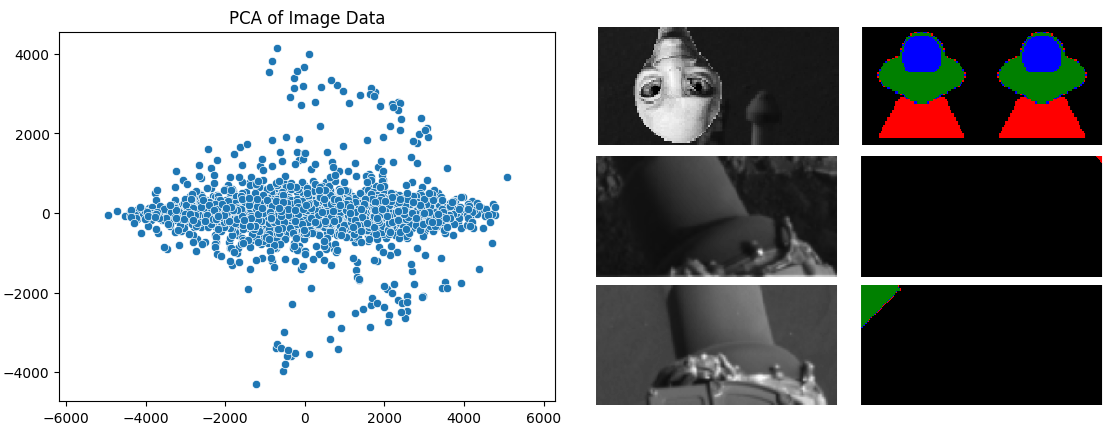
\includegraphics[width=0.9\linewidth]{images/initial_PCA.png}}
        % \centering
        % \caption{Initial PCA distribution and some examples of the samples removed}
        % \label{fig:fig1}
        % \end{figure}
        
        
        % See figure \ref{fig:fig2}

        % \begin{figure}[H]
        % \frame{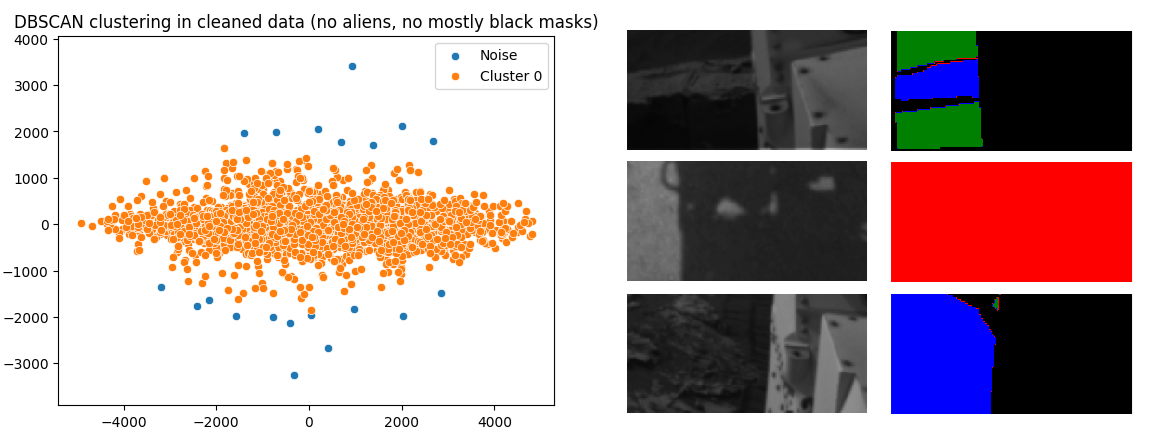
\includegraphics[width=0.9\linewidth]{images/DBSCAN1.png}}
        % \centering
        % \caption{DBSCAN distribution and aditional outliers}
        % \label{fig:fig2}
        % \end{figure}
        
        After the initial cleaning, DBSCAN \cite{ester1996density} was used.
        %a new distribution was computed to now identify additional outliers with DBSCAN.
        % It can be observed that the data distribution for cluster 0 (represented in orange) is more compact. 
        However, only 20 samples were classified as outliers, which are the images where the robot or its shadow obstructed the view. Despite this, some of these images contained valuable information, so a decision was made to retain them and preserve the first distribution.
        % seen on \ref{fig:fig2}.
        %(this is a parameter for the table (remove outliers=True)

        
        \subsection{Data Augmentation}
        \label{sec:aug}
        After the cleaning, this was the initial distribution of the classes: 

        \begin{table}[H]
        \begin{tabular}{|c|c|c|c|c|}
        \hline
        \rowcolor[HTML]{C0C0C0} 
        Class 0 & Class 1 & Class 2 & Class 3 & Class 4 \\ \hline
        20.52\% & 35.60\% & 24.44\% & 19.30\% & 0.14\%  \\ \hline
        \end{tabular}
        \end{table}
        
        Evidently, the dataset was highly unbalanced especially for class 4. To mitigate this problem, various data augmentation techniques were tried out, targeting specifically class 4 samples.

        \subsubsection{Augmenting only class 4 - Version 1}
        \label{sec:augv1}
        The process began by identifying a bounding box around the class 4 pixels in all the images where class 4 appeared, ensuring it met a minimum size. If the patch had sufficient coverage of class 4, it was cropped from the image and mask. The extracted region was then resized using interpolation to fit the target dimensions, maintaining the class distribution. The newly augmented class 4 samples were added to the dataset.
        \begin{figure}[H]
        \frame{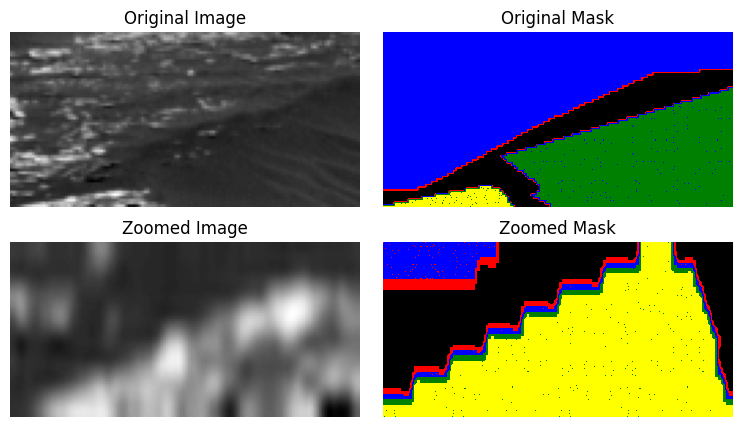
\includegraphics[width=0.8\linewidth]{images/aug1.png}}
        \centering
        \caption{Cropping and zooming augmentation}
        \label{fig:aug1}
        \end{figure}

        \subsubsection{Augmenting only class 4 - Version 2}
        \label{sec:augv2}
        This version of augmentation for class 4 starts with resizing and cropping the images and masks, just as in Version 1 \ref{sec:augv1}. This time the extracted patches are tiled together to create larger images that match the original size. 

        \begin{figure}[H]
        \frame{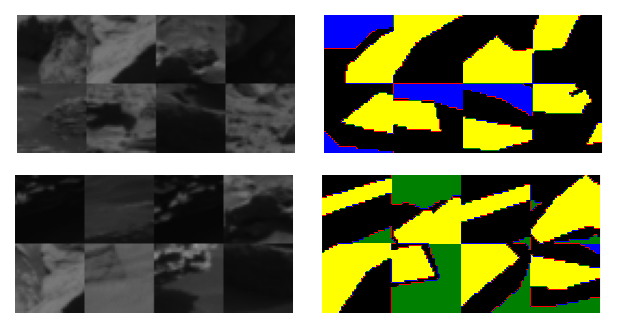
\includegraphics[width=0.8\linewidth]{images/aug2.png}}
        \centering
        \caption{Tiling augmentation}
        \label{fig:final_aug}
        \end{figure}

        \subsubsection{Augmenting only class 4 - Version 3}
        \label{sec:augv3}
         Since the samples extracted with the previous techniques seemed insufficient, light geometric and intensity transformations were applied to the images extracted for class 4 to increase diversity and representation coverage.

        \subsection{Model Design}

        Three model architectures were employed throughout this project, each one inspired from some state-of-the-art model for semantic segmentation problems. The first trials were made with a \textbf{U-Net} architecture \cite{ronneberger2015u}, which seemed the most reasonable choice to start experimenting. When the unbalanced nature of the dataset was revealed as the most important challenge to face in this project, other architectures were devised. First, \textbf{Attention U-Net} \cite{oktay2018attention} seemed to be a good solution as it is an extension of the original U-Net model, integrating an attention mechanism to focus on the most relevant regions of the input images during the skip connections. Second, \textbf{Dense U-Net} \cite{cai2020dense} was tested. The dense connectivity of this model and its improved feature propagation capabilities seemed more applicable to the domain of the problem.

        \subsection{Loss Function Design}
        Three different types of loss functions were tested, to assess the response of the model and cope with the imbalanced representation of class 4. The first and most straightforward approach was to apply \textbf{weighted categorical cross entropy}, which aims to focus more attention on the underrepresented classes by means of weights associated to each class. Then \textbf{dice loss}\cite{li2019dice} was implemented. It is derived from the Dice coefficient, which measures the overlap between predicted and ground truth region with an emphasis on small and underrepresented regions. Lastly \textbf{focal loss}\cite{ross2017focal} is used. It ends up being the best fit for our problem because it is designed to address class imbalance.

        
        
        %\textbf{U-Net} \cite{ronneberger2015u} architecture is a convolutional neural network designed primarily for the segmentation task on biomedical images. It has two symmetric key features, an encoder and a decoder. The encoder downsamples the input image following the traditional architecture of a convolutional network. Then, the decoder \textbf{upsamples} the features to reconstruct the segmented output. Further, it has introduced skip connections between the corresponding layers of the encoder and decoder. These connections enable the network to maintain the information during the upsampling phase. 
        %In our U-Net model, for the downsampling three 3x3 convolution layers are followed by a rectified linear unit (ReLU) and a 2x2 max pooling operation with stride 2. A total of 4 (depth) downsampling steps are applied, at each step, the number of feature channels is doubled. Following the downsampling, in the bottleneck 3 3x3 convolution layers are used with ReLU. Upsampling consists of a transpose layer that halves the number of feature channels, concatenation (skip connection) with the corresponding downsampling result, and three 3x3 convolutions followed by ReLU. Finally, a 1x1 convolution layer is used with a softmax activation function.
        
        
        
        %\textbf{Attention U-Net} \cite{oktay2018attention} extends U-Net architecture by implementing an attention mechanism to enhance the segmentation task, particularly for noisy datasets. The key feature of the Attention U-Net architecture is the attention gates (AGs). These gates filter the irrelevant information passed from the encoder to the decoder during the skip connections. 
        %Attention U-Net parameters are identical to the U-Net with an additional AG during skip connections. AG, upon receiving the corresponding encoder and decoder outputs, feeds them to a 1x1 convolution layer followed by a softmax activation creating an attention map that highlights the most relevant spatial locations. Then, the map is fed to another 1x1 convolution layer resulting in a refined attention map. AG outputs the encoder output multiplied by the refined attention map filtering the irrelevant information.
        
        
        
        %\textbf{Dense U-Net} \cite{cai2020dense} architecture is the same as U-Net architecture with only one key difference: in the encoder and decoder parts, each convolution layer is connected to every other layer, creating additional feature propagations. This connection allows the model to learn more robust features with fewer parameters by improving gradient flow.
        %After each convolution block, the result and the initial input to the convolution block are concatenated and passed to the following blocks. \\

        
        %Lastly, an \textbf{ensemble method} was implemented. The main goal of this ensemble model is to train a specific model to segment the background from the other objects. Currently, the models are not labelling any pixel as background since the weight of the background is set to 0. Therefore, combining a background-specific model with the current best models should yield better results by reducing the wrong segmentations. The prediction of the ensemble model is 0 (background) if the background-specific model predicts 0; the prediction of the main model does not change if the background-specific model predicts 1 (object).


    \section{Experiments}
        \textbf{Early experiments:}
        The experimentation started with the simplest model design and no modifications on the dataset to assess the complexity of the task and the baseline. A U-Net model was trained on the original dataset with sparse categorial cross-entropy and Dice loss functions. This baseline turned out to be quite good, with almost 52\% accuracy on the test set.

        %Thanks to these first experiments we discovered the presence of the outliers described in section \ref{sec:wrangling}. 
        
        \textbf{Mid-stage experiments:}
        After cleaning the data set, data augmentation was tried out on the entire dataset, but there was no big improvement. Therefore, a more in-depth data inspection process started. This analysis showed that class 4 was severely underrepresented and was hindering the learning process of the model drastically. 
        %The model was correctly learning how to segment classes 1, 2 and 3, but it was achieving very low IoU results for class 4, leading to a poor mean overall. 
        It also showed that the background was predominant in the dataset, leading to confusion in the learning process.

        To cope with these, augmentation techniques were designed specifically for class 4.
        %to tackle the under representation of class 4. 
        Additionally, the weight associated to the background class was  set to 0, to force the model to stop learning background segmentation.
        %prevent the model to focus on learning how to classify the background correctly (as it was the most represented class).
        The results coming from these changes in the approach were promising, leading to a mean IoU of 67\% over the test set. This was achieved with Dense U-Net, and the dataset enhanced for class 4 representation balancing.
        
        \textbf{Late experiments:}
         At this point minor adjustments were done to every strategy adopted throughout the process; removing some extra outliers or data samples for balancing the dataset; trying different types of augmentation for class 4 and combining them; playing with the weights associated to the classes; and trying different combinations of models and loss functions.
         Not every combination of these techniques achieved great results, but throughout this period of trials multiple attempts scored high, between 68\% and 70\% mean IoU (over the test set), leading to the highest results for the project.
        
        
    \section{Results}

% Please add the following required packages to your document preamble:
% \usepackage[table,xcdraw]{xcolor}
% Beamer presentation requires \usepackage{colortbl} instead of \usepackage[table,xcdraw]{xcolor}

\begin{table}[H]
\resizebox{0.5\textwidth}{!}{\begin{tabular}{|r|c|c|c|c|}
\hline
\rowcolor[HTML]{C0C0C0} 
\textbf{Model}                                             & \textbf{Augmentation}                                                                                 & \textbf{Loss Function}                                                                             & \textbf{\begin{tabular}[c]{@{}c@{}}Local \\ Mean IOU\end{tabular}} & \textbf{\begin{tabular}[c]{@{}c@{}}Kaggle \\ Result\end{tabular}} \\ \hline
\rowcolor[HTML]{DAE8FC} 
U-Net                                                      & \begin{tabular}[c]{@{}c@{}}Unclean data\\ No augmentation\end{tabular}                                & Dice Loss                                                                                          & 0.5094                                                             & 0.5191                                                   \\ \hline
\rowcolor[HTML]{ECF4FF} 
\begin{tabular}[c]{@{}r@{}}Attention \\ U-Net\end{tabular} & \begin{tabular}[c]{@{}c@{}}Clean Data\\ Only Class 4 \\ Version1\end{tabular}                         & \begin{tabular}[c]{@{}c@{}}Weighted \\ Categorical \\ Crossentropy\end{tabular}                    & {\color[HTML]{333333} 0.5560}                                      & 0.6654                                                            \\ \hline
\rowcolor[HTML]{DAE8FC} 
\begin{tabular}[c]{@{}r@{}}Dense \\ U-Net\end{tabular}     & \cellcolor[HTML]{DAE8FC}\begin{tabular}[c]{@{}c@{}}Clean Data\\ Only Class 4 \\ Version2\end{tabular} & Focal Loss                                                                                         & 0.663                                                              & \textbf{0.7055}                                                   \\ \hline

\rowcolor[HTML]{ECF4FF} 
\begin{tabular}[c]{@{}r@{}}Dense \\ U-Net\end{tabular}     & \begin{tabular}[c]{@{}c@{}}Clean\\ Only Class 4 \\ Version3\end{tabular}                              & \begin{tabular}[c]{@{}c@{}}Weighted \\ Categorical \\ Crossentropy\end{tabular}                    & {\color[HTML]{333333} \textbf{0.6525}}                             & 0.6854                                                   \\ \hline
\end{tabular}}
\caption{Some of the results. All the models, except the first one, sets background weight zero.}\label{table:results}
\end{table}

The most significant results are presented in Table \ref{table:results}. All the detailed results are in the Appendix \ref{sec:apx} Table \ref{table:appx}. The best result is achieved by Dense U-Net using only class 4 augmentation (version 2), focal loss and setting background weights to 0 with the Mean Intersection over Union (Mean IoU) score of \textbf{70.55\%} on Kaggle test data. Overall, considering the other augmentation versions, \textbf{Dense U-Net} performs better than Attention U-Net. Furthermore, the models perform better with \textbf{focal loss} compared to dice loss and weighted categorical crossentropy. Focal loss is mathematically designed to discourage the model to keep learning on classes that already have high accuracy. As a consequence of this, it managed to drive the model’s attention to classify correctly class 4 pixels, even if they were the minority of the original dataset.

% The results obtained by applying this loss function were underwhelming, as it was not able to even out the learning process over such an unbalanced dataset.

    
    \section{Discussion}

    The final results obtained showed that it is not always necessary to have a really large and correctly labeled dataset in order to achieve high scores and metrics for a semantic segmentation problem. This is possible thanks to fully convolutional neural networks such as U-Net. Despite all of this, a well-designed dataset, with a larger amount of samples and correctly labeled masks would have most likely improved the prediction power of the model.
    %Another consideration that can be made, is related to the use of pre-trained models for transfer learning and fine-tuning. The use of pre-trained models might boost even further the performance achieved in this project, if correctly employed.

        

    \section{Conclusions}
      In this assignment, we worked on a segmentation problem with images from the Mars terrain. Having a highly unbalanced dataset, most of the effort was put into augmentation. Three types of augmentation, three different model architectures, and three different types of loss functions were implemented. Out of all these combinations, the best results were achieved with the augmentation techniques applied for class 4 and the Dense U-Net architecture with focal loss, scoring a mean IoU of 70.5\% over the test set. 
      
        In future work, the given dataset maybe analyzed further, since the correctness of the given masks was constantly questioned and was a recurrent problem throughout the process. It is also possible to further investigate possible ensemble models and hybrid loss functions.


    
   
    
    \section{Team contributions}
    
    \textbf{Sergio} focused on data wrangling and implementing initial data analysis distribution. \textbf{Pinar} worked on the building the base U-Net, dense U-Net and ensemble models. \textbf{Angela} contributed by building the attention U-Net approach and class balancing functions. The augmentation techniques for class 4 for class balancing were created by \textbf{Matteo}, who also analyzed the performance of different loss functions.
    % \textbf{All team members} collaborated on the report of the project and contributed equally ensuring a balanced workload and a cohesive submission.

    
    % \clearpage
    
% \FloatBarrier
% \begin{table*}[ht!]
%  \hskip-1.5cm
% \begin{tabular}{lccc|cccc|c|}
% \cline{5-9}
%                                                                                      & \multicolumn{1}{l}{}                                       & \multicolumn{1}{l}{}                                               & \multicolumn{1}{l|}{} & \multicolumn{4}{c|}{\cellcolor[HTML]{C0C0C0}Local Results}                                                                                                                                                      & \multicolumn{1}{l|}{\cellcolor[HTML]{C0C0C0}CodaBench} \\ \hline
% \rowcolor[HTML]{C0C0C0} 
% \multicolumn{1}{|l|}{\cellcolor[HTML]{C0C0C0}\textbf{Model}}                         & \multicolumn{1}{c|}{\cellcolor[HTML]{C0C0C0}\textbf{Data}} & \multicolumn{1}{c|}{\cellcolor[HTML]{C0C0C0}\textbf{Augmented}} & \textbf{Fine-tuning}  & \multicolumn{1}{c|}{\cellcolor[HTML]{C0C0C0}\textbf{Accuracy}} & \multicolumn{1}{c|}{\cellcolor[HTML]{C0C0C0}\textbf{Precision}} & \multicolumn{1}{c|}{\cellcolor[HTML]{C0C0C0}\textbf{Recall}} & \textbf{F1}   & \textbf{Accuracy}                                      \\ \hline
% \multicolumn{1}{|l|}{Base Model}                                                     & \multicolumn{1}{c|}{Unclean}                               & \multicolumn{1}{c|}{No}                                            & No                    & \multicolumn{1}{c|}{0.7}                                       & \multicolumn{1}{c|}{0.72}                                       & \multicolumn{1}{c|}{0.7}                                     & 0.68          & 0.14                                                   \\ \hline
% \multicolumn{1}{|l|}{VGG}                                                            & \multicolumn{1}{c|}{Clean}                                 & \multicolumn{1}{c|}{No}                                            & Yes                   & \multicolumn{1}{c|}{0.87}                                      & \multicolumn{1}{c|}{0.91}                                       & \multicolumn{1}{c|}{0.87}                                    & 0.88          & 0.49                                                   \\ \hline
% \multicolumn{1}{|l|}{ConvNextBase}                                                   & \multicolumn{1}{c|}{Clean}                                 & \multicolumn{1}{c|}{Yes}                                           & Yes                   & \multicolumn{1}{c|}{0.97}                                      & \multicolumn{1}{c|}{0.97}                                       & \multicolumn{1}{c|}{0.97}                                    & 0.97          & 0.85                                          \\ \hline
% \multicolumn{1}{|l|}{ConvNextLarge}                                                  & \multicolumn{1}{c|}{Clean}                                 & \multicolumn{1}{c|}{Yes}                                           & Yes                   & \multicolumn{1}{c|}{0.98}                             & \multicolumn{1}{c|}{0.98}                              & \multicolumn{1}{c|}{0.98}                           & 0.98 & 0.85                                          \\ \hline
% \multicolumn{1}{|l|}{ConvNextXLarge}                                                 & \multicolumn{1}{c|}{Clean}                                 & \multicolumn{1}{c|}{No}                                            & No                    & \multicolumn{1}{c|}{0.95}                                      & \multicolumn{1}{c|}{0.95}                                       & \multicolumn{1}{c|}{0.95}                                    & 0.95          & 0.74                                                   \\ \hline
% \multicolumn{1}{|l|}{ConvNextXLarge}                                                 & \multicolumn{1}{c|}{Clean}                                 & \multicolumn{1}{c|}{Yes}                                           & Yes                   & \multicolumn{1}{c|}{0.98}                                          & \multicolumn{1}{c|}{0.98}                                           & \multicolumn{1}{c|}{0.98}                                        & 0.98              & \textbf{0.87}                                                       \\ \hline
% \multicolumn{1}{|l|}{\begin{tabular}[c]{@{}l@{}}Block\\ ConvNextXlarge\end{tabular}} & \multicolumn{1}{c|}{Clean}                                 & \multicolumn{1}{c|}{Yes}                                           & Yes                   & \multicolumn{1}{c|}{0.99}                                          & \multicolumn{1}{c|}{0.99}                                           & \multicolumn{1}{c|}{0.99}                                        & 0.99              &    0.79                                                    \\ \hline
% \end{tabular}
%         \caption{Summary of the models' performances}
%         % \label{tab:Performance}
% \end{table*}




% \FloatBarrier        


        


    \bibliography{references}
    \bibliographystyle{abbrv}

    

    
    
    
    
    \end{multicols}
        
    \clearpage
    
\section{Apendix}
\label{sec:apx}
%Useful conventions to read the following table:
%\begin{itemize}
%    \item LMIOU: Local Mean IOU (Table header)
%    \item KR: Kaggle Result (Table header)
%    \item BG: Background
%    \item AU-Net: Attention U-Net (Model Column)
%    \item WCC: Weighted Categorical Crossentropy (Loss Funcion Column)
%    \item *: (Removed some data for balancing)
%    \item **: Remove Outliers
%\end{itemize}
\begin{table}[H]
\begin{tabular}{|r|c|c|c|c|c|c|}
\hline
\rowcolor[HTML]{C0C0C0} 
\textbf{Model}                                                                               & \textbf{Data}                                                                        & \textbf{Augmentation}                                            & \textbf{Loss Function}                                                                             & \textbf{Class Weights}                                                         & \textbf{LMIOU}                                & \textbf{KR}   \\ \hline
\rowcolor[HTML]{DAE8FC} 
U-Net                                                                                        & Unclean                                                                              & No                                                               & \begin{tabular}[c]{@{}c@{}}Sparse Categorical \\ Crossentropy\end{tabular}                         & N/A                                                                            & 0.4176                                                 & 0.4299                   \\ \hline
\rowcolor[HTML]{DAE8FC} 
Dense U-Net                                                                                  & Unclean                                                                              & No                                                               & Dice Loss                                                                                          & N/A                                                                            & 0.4829                                                 & 0.47964                  \\ \hline
\rowcolor[HTML]{DAE8FC} 
U-Net                                                                                        & Unclean                                                                              & No                                                               & Dice Loss                                                                                          & N/A                                                                            & 0.5094                                                 & \textbf{0.5191}          \\ \hline
\rowcolor[HTML]{DAE8FC} 
U-Net                                                                                        & Clean                                                                                & No                                                               & Dice Loss                                                                                          & BG weight = 0                                                          & 0.5609                                                 & 0.4899                   \\ \hline
\rowcolor[HTML]{DAE8FC} 
U-Net                                                                                        & Clean                                                                                & No                                                               & Focal Loss                                                                                         & BG weight = 0                                                          & \textbf{0.5166}                                        & 0.4834                   \\ \hline
\rowcolor[HTML]{ECF4FF} 
AU-Net                                                                              & Clean                                                                                & All classes                                                        & Dice Loss                                                                                          & N/A                                                                            & 0.5086                                                 & 0.5002                   \\ \hline
\rowcolor[HTML]{ECF4FF} 
AU-Net                                                                              & Clean                                                                                & All classes                                                        & Dice Loss                                                                                          & BG weight = 0                                                          & 0.4270                                                 & 0.4166                   \\ \hline
\rowcolor[HTML]{ECF4FF} 
AU-Net                                                                              & Clean                                                                                & \begin{tabular}[c]{@{}c@{}}Only Class 4 (V1)\end{tabular} & \begin{tabular}[c]{@{}c@{}}WCC\end{tabular}                       & BG weight = 0                                                          & 0.5560                                                 & 0.6654                   \\ \hline
\rowcolor[HTML]{ECF4FF} 
AU-Net                                                                              & Clean                                                                                & \begin{tabular}[c]{@{}c@{}}Only Class 4 (V1)\end{tabular} & \begin{tabular}[c]{@{}c@{}}WCC\end{tabular}                       & \begin{tabular}[c]{@{}c@{}}Normalized\\ BG weight = 0\end{tabular}     & 0.5405                                                 & 0.6190                   \\ \hline
\rowcolor[HTML]{ECF4FF} 
Dense U-Net                                                                                  & Clean                                                                                & \begin{tabular}[c]{@{}c@{}}Only Class 4 (V1)\end{tabular} & \begin{tabular}[c]{@{}c@{}}WCC\end{tabular}                       & BG weight = 0                                                          & \textbf{0.57}                                          & \textbf{0.6753}          \\ \hline
\rowcolor[HTML]{DAE8FC} 
U-Net                                                                                        & Clean                                                                                & \begin{tabular}[c]{@{}c@{}}Only Class 4 (V2)\end{tabular} & \begin{tabular}[c]{@{}c@{}}WCC\end{tabular}                       & BG weight = 0                                                          & 0.5868                                                 & 0.5690                   \\ \hline
\rowcolor[HTML]{DAE8FC} 
AU-Net                                                                              & \begin{tabular}[c]{@{}c@{}}Clean*\end{tabular} & \begin{tabular}[c]{@{}c@{}}Only Class 4 (V2)\end{tabular} & \begin{tabular}[c]{@{}c@{}}WCC\end{tabular}                       & \begin{tabular}[c]{@{}c@{}}All balanced\\ BG weight = 0\end{tabular}   & 0.5163                                                 & 0.5811                   \\ \hline
\rowcolor[HTML]{DAE8FC} 
AU-Net                                                                              & Clean                                                                                & \begin{tabular}[c]{@{}c@{}}Only Class 4 (V2)\end{tabular} & \begin{tabular}[c]{@{}c@{}}WCC\end{tabular}                       & BG weight = 0                                                          & 0.5943                                                 & 0.6019                   \\ \hline
\rowcolor[HTML]{DAE8FC} 
Dense U-Net                                                                                  & Clean                                                                                & \begin{tabular}[c]{@{}c@{}}Only Class 4 (V2)\end{tabular} & \begin{tabular}[c]{@{}c@{}}WCC\end{tabular}                       & BG weight = 0                                                          & 0.6602                                                 & 0.6876                   \\ \hline
\rowcolor[HTML]{DAE8FC} 
Dense U-Net                                                                                  & Clean                                                                                & \begin{tabular}[c]{@{}c@{}}Only Class 4 (V2)\end{tabular} & \begin{tabular}[c]{@{}c@{}}WCC\end{tabular}                       & \begin{tabular}[c]{@{}c@{}}Normal weights\end{tabular}             & {\cellcolor[HTML]{EE4B2B} \textbf{0.7821}}                 & 0.5224                   \\ \hline
\rowcolor[HTML]{DAE8FC} 
\begin{tabular}[c]{@{}r@{}}Ensemble:\\ BG AU-Net\\ Dense U-Net\end{tabular} & Clean                                                                                & \begin{tabular}[c]{@{}c@{}}Only Class 4 (V2)\end{tabular} & \begin{tabular}[c]{@{}c@{}}Binary Crossentropy\\ WCC\end{tabular} & \begin{tabular}[c]{@{}c@{}}Binary weights\\ BG weight = 0\end{tabular} & \begin{tabular}[c]{@{}c@{}}0.515\\ 0.6602\end{tabular} & 0.6315                   \\ \hline
\rowcolor[HTML]{DAE8FC} 
Dense U-Net                                                                                  & Clean                                                                                & \begin{tabular}[c]{@{}c@{}}Only Class 4 (V2)\end{tabular} & Dice Loss                                                                                          & N/A                                                    & 0.768                                                  & 0.5354                   \\ \hline
\rowcolor[HTML]{DAE8FC} 
Dense U-Net                                                                                  & Clean                                                                                & \begin{tabular}[c]{@{}c@{}}Only Class 4 (V2)\end{tabular} & Focal Loss                                                                                         & BG weight = 0                                  & 0.663                                                  & {\cellcolor[HTML]{7CFC00}\textbf{0.7055}}          \\ \hline
\rowcolor[HTML]{DAE8FC} 
Dense U-Net                                                                                  & Clean                                                                                & \begin{tabular}[c]{@{}c@{}}Only Class 4 (V2)\end{tabular} & \cellcolor[HTML]{DAE8FC}Focal Loss                                                                 & \cellcolor[HTML]{DAE8FC}BG weight = 0.1                                & 0.6944                                                 & 0.5580                   \\ \hline
\rowcolor[HTML]{ECF4FF} 
Dense U-Net                                                                                  & Clean                                                                                & \begin{tabular}[c]{@{}c@{}}Only Class 4 (V3)\end{tabular} & \begin{tabular}[c]{@{}c@{}}WCC\end{tabular}                       & BG weight = 0                                                          & 0.6525                                                 & \textbf{0.6854}          \\ \hline
\rowcolor[HTML]{ECF4FF} 
AU-Net                                                                              & Clean                                                                                & \begin{tabular}[c]{@{}c@{}}Only Class 4 (V3)\end{tabular} & \begin{tabular}[c]{@{}c@{}}WCC\end{tabular}                       & BG weight = 0                                                          & 0.6374                                                 & 0.6221                   \\ \hline
\rowcolor[HTML]{ECF4FF} 
Dense U-Net                                                                                  & \begin{tabular}[c]{@{}c@{}}Clean**\end{tabular}                      & \begin{tabular}[c]{@{}c@{}}Only Class 4 (V3)\end{tabular} & \begin{tabular}[c]{@{}c@{}}WCC\end{tabular}                       & \begin{tabular}[c]{@{}c@{}}Normal weights\end{tabular}             & {\cellcolor[HTML]{EE4B2B} \textbf{0.8264}}                 & 0.5253                   \\ \hline
\rowcolor[HTML]{ECF4FF} 
Dense U-Net                                                                                  & \begin{tabular}[c]{@{}c@{}}Clean\end{tabular}                      & \begin{tabular}[c]{@{}c@{}}Only Class 4 (V3)\end{tabular} & \begin{tabular}[c]{@{}c@{}}Focal Loss\end{tabular}                       & \begin{tabular}[c]{@{}c@{}}BG weight = 0\end{tabular}             & 0.6535                 & 0.6902                \\ \hline
\end{tabular}
\caption{Results of all the models. Red ones indicate a possible overfit and green is the best result(\textbf{LMIOU}: Local Mean IOU, 
     \textbf{KR}: Kaggle Result,
     \textbf{BG}: Background,
    \textbf{AU-Net:} Attention U-Net,
    \textbf{WCC}: Weighted Categorical Crossentropy,
    \textbf{*:} Removed some data for balancing,
    \textbf{**:} Remove Outliers)} \label{table:appx}
\end{table}
\end{document}